%%%%%%%%%%%%%%%%%%%%%%%%%%%%%%%%%%%%%%%%%
%
% This template is based on a template by:
% Steve Gunn (http://users.ecs.soton.ac.uk/srg/softwaretools/document/templates/)
% Sunil Patel (http://www.sunilpatel.co.uk/thesis-template/)
%
% Template license:
% CC BY-NC-SA 3.0 (http://creativecommons.org/licenses/by-nc-sa/3.0/)
%
%%%%%%%%%%%%%%%%%%%%%%%%%%%%%%%%%%%%%%%%%

%----------------------------------------------------------------------------------------
%	CONFIGURATION
%----------------------------------------------------------------------------------------

\documentclass[
12pt, 
french, 
singlespacing,
headsepline,
]{Analyse}

\usepackage[utf8]{inputenc}
\usepackage[T1]{fontenc}

\usepackage{mathpazo}

\usepackage[backend=bibtex,style=authoryear,natbib=true]{biblatex}

\addbibresource{bibliographie}

\usepackage[autostyle=true]{csquotes}

%----------------------------------------------------------------------------------------
%	MARGE
%----------------------------------------------------------------------------------------

\geometry{
	paper=a4paper, 
	inner=2.5cm, 
	outer=3.8cm, 
	bindingoffset=.5cm, 
	top=1.5cm, 
	bottom=1.5cm,
}

%----------------------------------------------------------------------------------------
%	INFORMATIONS
%----------------------------------------------------------------------------------------

\thesistitle{Analyse Publicitaire}
\author{Alexandre \textsc{GERARD}}

\subject{Expression-Communication}
\university{\href{http://iut-metz.univ-lorraine.fr}{Université de Lorraine}}
\department{\href{http://iut-metz.univ-lorraine.fr}{Département Informatique}}
\group{IP GRP 2}

\AtBeginDocument{
\hypersetup{pdftitle=\ttitle}
\hypersetup{pdfauthor=\authorname}
\hypersetup{pdfkeywords=\keywordnames}
}

\begin{document}

\frontmatter

\pagestyle{plain}

%----------------------------------------------------------------------------------------
%	TITRE
%----------------------------------------------------------------------------------------

\begin{titlepage}
\begin{center}

\vspace*{.05\textheight}
{\scshape\LARGE \univname\par}\vspace{1.5cm}
\textsc{\Large Expression-Communication}\\[0.5cm]

\HRule \\[0.4cm]
{\huge \bfseries \ttitle\par}\vspace{0.4cm}
\HRule \\[1.5cm]
 
\begin{minipage}[t]{1\textwidth}
\begin{center} \large
\emph{Auteur:}\\
\href{https://agerard57.github.io/}{\authorname}
\end{center}
\end{minipage}
\begin{minipage}[t]{0.4\textwidth}
\end{minipage}\\[3cm]
 
\vfill

\large \textit{Analyse poussée d'une publicité extraite d'une campagne \\ venant d'une marque à notoriété mondiale }\\[0.3cm]
\vspace*{15mm}
\groupname\\\deptname\\[2cm]

\includegraphics[width=20mm]{medias/ul.png}

\vfill

{\large \today}\\[4cm]

 
\vfill
\end{center}
\end{titlepage}

%----------------------------------------------------------------------------------------
%	TABLES DES MATIÈRES
%----------------------------------------------------------------------------------------

\tableofcontents

%----------------------------------------------------------------------------------------
%	CONTENU
%----------------------------------------------------------------------------------------

\mainmatter
\pagestyle{analyse}

\chapter{Introduction}

\label{Introduction}

\section{Coca-cola, une emprise mondiale}

Afin de pouvoir analyser une publicité de façon efficace, j'ai décidé de directement analyser les techniques de commercialisation mis en place par la \textit{Coca-Cola Company}.
En effet, c'est en 2012 que la marque mondialement connue atteint de nouveaux sommets et devance tous ses concurrents avec des revenus de près de \textbf{48 milliards de dollars}.  Jusqu'à lors, c'était \textit{PepsiCo} qui menait le marché.
Or, le succès de Coca-Cola provient, sans aucun doute, de ces multiples réclames et campagnes publicitaires, qui, même après être passés premiers mondiaux, continuent de pulluler dans la rue, sur nos télés, nos téléphones, etc.\\
Coca-Cola n'hésite pas à investir des sommes colossales dans la réclame et la communication (avec un budget de plus de 2 milliards de dollars par an). Leur publicités se déclinent en images fortes qui ont su s'imprimer dans la conscience collective, que ce soit avec leur ours de synthèse, avec le Père Noël ou encore par des stratégies connotés "classiques", stimulant les pulsions primaires (par exemple la soif ou la sexualité…). \parencite{Ref1}. \\


\hfill \break

\begin{figure}[th]
\centering
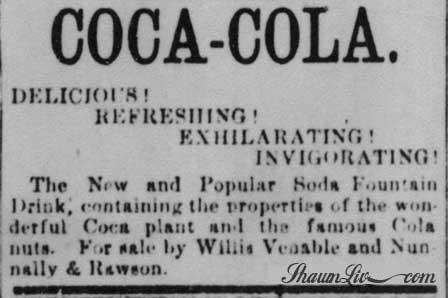
\includegraphics[width=100mm]{medias/1ere_pub}
\decoRule
\caption{1886, Atlanta - Première publicité coca-cola}
\end{figure}
\newpage

%----------------------------------------------------------------------------------------


\section{Introduction de la campagne }

Parmi les campagnes les plus célèbres que coca-cola ait publiés, j'ai choisi de me pencher sur un précurseur de la marque, une campagne qui à tellement fait parler d'elle, qu'encore aujourd'hui les gens en parlent encore et vont jusqu'à penser que le Père Noël est le fruit de la compagnie;  il s'agit de la campagne à grande échelle "\textit{coke x-mas}".
Cette campagne à vu le jour en décembre 1930, à cette période là, coca-cola était une boisson gazeuse locale aux Américains, exclusivement réservée aux périodes estivales.
Voulant "rafraîchir" et étendre la marque, cette campagne eu alors deux objectifs : 

\begin{itemize}
\item Trouver un moyen, avec une image ou un symbole mondialement connu, de s'exporter ;
\item Couvrir plus de saisons, afin d'augmenter les ventes;
\end{itemize}

\begin{figure}[th]
\centering

\includegraphics[width=70mm]{medias/perenoel1}

\includegraphics[width=70mm]{medias/perenoel2}
\decoRule
\caption{1935/1361 - Quelques réclames de la campagne "coke x-mas"}
\end{figure}

\chapter{Analyse d'une des publicités}

\label{Analyse d'une des publicités}

\section{Présentation de la publicité analysée}

De ce contexte, né en 1964, de la plume de l'illustrateur New-Yorkais \textit{Haddon Sundblom}, la réclame qui nous intéresse.

\begin{figure}[th]
\centering
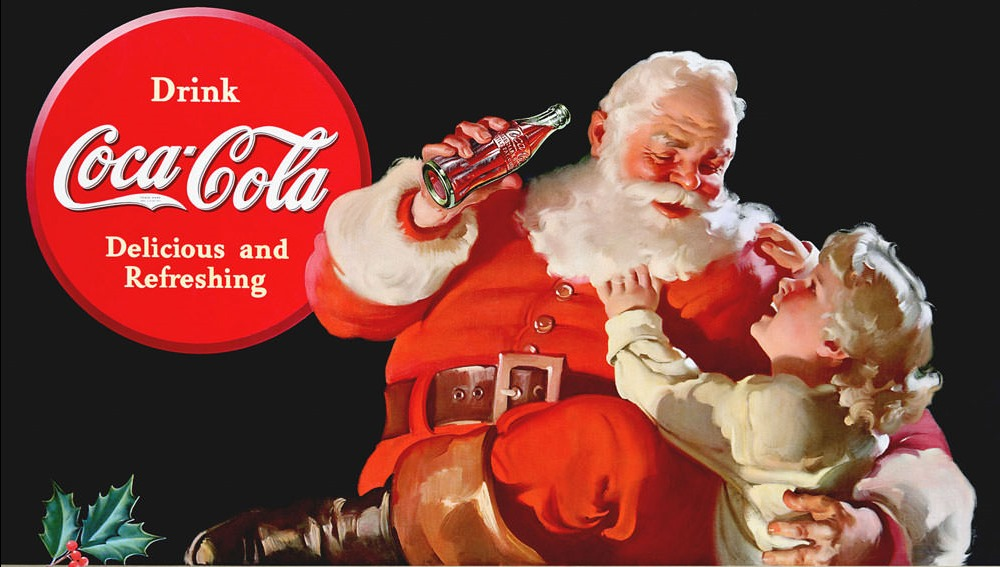
\includegraphics[width=130mm]{medias/affiche_coca}
\decoRule
\caption{Réclame étudiée dans cette partie.}
\end{figure}

J'ai choisi cette publicité en particulier car elle résume en idées simples tout les messages que l'entreprise souhaitait faire passer pendant cette période de son histoire.

%----------------------------------------------------------------------------------------

\section{Analyse descriptive de la publicité}

\subsection{Une présentation sobre}
On voit tout d'abord qu'il n'y a aucun élément superflu, le fond est noir, ce qui nous fait comprendre que cette réclame veut uniquement montrer ce qu'elle a à dire, mettant d'avantage en avant ses propos. Tout élément ici a donc son importance; À première vue, on remarque entre-autres, trois éléments principaux dans la composition: le père noël, ayant une place centrale quoique légèrement déportée par la droite afin de laisser place au logo coca-cola, dans un cercle rouge avec deux slogans. On pourrait aller jusqu'à formaliser et penser que l'utilisation du cercle rouge n'est pas dû à un simple hasard mais bien au rappel des capsules de bouteilles en verre, renforçant d'avantage de façon non-consciente la marque dans nos esprits.
\subsection{Une présentation attrayante}
Le fond noir ne sert pas qu'à mettre en avant les éléments, mais fait même mieux ressortir les couleurs prédominantes de la marque. On remarque que tout est aussi fait pour associer le bonheur avec la boisson, en particulier avec le sourire des personnages.
\subsection{Un rappel des thèmes hivernaux}

%----------------------------------------------------------------------------------------

\section{Le but de la publicité}

\subsection{"\textit{Drink Coke}"}
Il faut avant tout savoir quel est le but de cette opération; En effet, on peut grossièrement catégoriser les types de publicités en trois catégories, toutes aux ambitions bien différentes :
\renewcommand{\labelitemi}{$\bullet$}
\begin{itemize}
\item La publicité argumentation : elle défend une idée et/ou tente de modifier l’opinion des récepteurs.
\item La publicité informative : elle a pour fonction de livrer au récepteur une information.
\item La publicité incitative : ce type de publicités poussent les gens à agir et à acheter un produit
\end{itemize}
On remarque que la stratégie commerciale qu'emploie Coca-Cola tient de l'ordre de la publicité incitative:
on le remarque tout d'abord dans ce qui était leur slogan que l'on retrouve sur cette publicité, "\textit{Drink Coca-Cola.}" ("\textit{Bois Coca-Cola.}"), qui ressemble fortement à une sorte d'ordre voire d'injonction que le consommateur reçoit. De plus, on remarque que cette méthode agressive transparaît aussi dans d'autres slogans, comme par exemple en 1952 avec "\textit{What you want is a Coke.}" ("\textit{Ce que vous avez besoin, c'est d'un Coca-Cola.}").
On cherche donc à aguicher le consommateur par 
\chapter{Conclusion}

\label{Conclusion}

\section{Coca-cola, une emprise mondiale}

La publicité a une influence sur les consommateurs lorsqu’elle est bien conçue. Le dilemme est de faire réagir ceux qui n’ont pas du tout envie de le faire même après avoir pris connaissance d’une information. C’est la raison pour laquelle il faut peser ses mots et utiliser les bons mots pour atteindre efficacement la cible.

\hfill \break


%----------------------------------------------------------------------------------------

\begin{flushright}
Analyse faite par ---\\
GERARD Alexandre: \href{https://agerard57.github.io/}{https://agerard57.github.io/}\\
Mail: \href{mailto:agerard57@protonmail.com}{agerard57@protonmail.com}
\end{flushright}


%----------------------------------------------------------------------------------------
%	BIBLIOGRAPHIE
%----------------------------------------------------------------------------------------

\printbibliography[heading=bibintoc]

%----------------------------------------------------------------------------------------

\end{document}  
